\PassOptionsToPackage{unicode=true}{hyperref} % options for packages loaded elsewhere
\PassOptionsToPackage{hyphens}{url}
%
\documentclass[12pt,english,]{article}
\usepackage{lmodern}
\usepackage{amssymb,amsmath}
\usepackage{ifxetex,ifluatex}
\usepackage{fixltx2e} % provides \textsubscript
\ifnum 0\ifxetex 1\fi\ifluatex 1\fi=0 % if pdftex
  \usepackage[T1]{fontenc}
  \usepackage[utf8]{inputenc}
  \usepackage{textcomp} % provides euro and other symbols
\else % if luatex or xelatex
  \usepackage{unicode-math}
  \defaultfontfeatures{Ligatures=TeX,Scale=MatchLowercase}
\fi
% use upquote if available, for straight quotes in verbatim environments
\IfFileExists{upquote.sty}{\usepackage{upquote}}{}
% use microtype if available
\IfFileExists{microtype.sty}{%
\usepackage[]{microtype}
\UseMicrotypeSet[protrusion]{basicmath} % disable protrusion for tt fonts
}{}
\usepackage{hyperref}
\hypersetup{
            pdfborder={0 0 0},
            breaklinks=true}
\urlstyle{same}  % don't use monospace font for urls
\usepackage[margin=1in]{geometry}
\usepackage{graphicx,grffile}
\makeatletter
\def\maxwidth{\ifdim\Gin@nat@width>\linewidth\linewidth\else\Gin@nat@width\fi}
\def\maxheight{\ifdim\Gin@nat@height>\textheight\textheight\else\Gin@nat@height\fi}
\makeatother
% Scale images if necessary, so that they will not overflow the page
% margins by default, and it is still possible to overwrite the defaults
% using explicit options in \includegraphics[width, height, ...]{}
\setkeys{Gin}{width=\maxwidth,height=\maxheight,keepaspectratio}
\setlength{\emergencystretch}{3em}  % prevent overfull lines
\providecommand{\tightlist}{%
  \setlength{\itemsep}{0pt}\setlength{\parskip}{0pt}}
\setcounter{secnumdepth}{0}
% Redefines (sub)paragraphs to behave more like sections
\ifx\paragraph\undefined\else
\let\oldparagraph\paragraph
\renewcommand{\paragraph}[1]{\oldparagraph{#1}\mbox{}}
\fi
\ifx\subparagraph\undefined\else
\let\oldsubparagraph\subparagraph
\renewcommand{\subparagraph}[1]{\oldsubparagraph{#1}\mbox{}}
\fi

% set default figure placement to htbp
\makeatletter
\def\fps@figure{htbp}
\makeatother

\usepackage{float}
\usepackage[boxruled,vlined]{algorithm2e}
\usepackage{listings}
\usepackage{xcolor}
\usepackage {tikz}
\usepackage{indentfirst}
\usepackage{tabularx}
\usepackage{multirow}
\usepackage{pgfplots}
\usepackage{wrapfig}
\usepackage{booktabs,makecell}
%\usepackage[bottom]{footmisc}
\colorlet{mygray}{black!30}
\colorlet{mygreen}{green!60!black}
\colorlet{mymauve}{red!90}

\lstset{
  tabsize=2,
  backgroundcolor=\color{gray!10},  
  basicstyle=\ttfamily,
  columns=fullflexible,
  breakatwhitespace=false,      
  breaklines=true,                
  captionpos=b,                    
  commentstyle=\color{mygreen}, 
  extendedchars=true,              
  frame=single,                   
  keepspaces=true,             
  keywordstyle=\bfseries\color{blue},      
  language=c++,                 
  numbers=left,                
  numbersep=5pt,
  breaklines=true,
  numberstyle=\tiny, 
  rulecolor=\color{mygray},        
  showspaces=false,               
  showtabs=true,                                  
  stringstyle=\color{mymauve},                          
  title=\lstname                
}

\definecolor{light-gray}{gray}{0.9}
\newcommand{\code}[1]{\colorbox{light-gray}{\texttt{#1}}}
\newcommand{\pnt}[1]{{\scriptstyle#1}}
\let\origfigure\figure
\let\endorigfigure\endfigure
\renewenvironment{figure}[1][2] {
    \expandafter\origfigure\expandafter[H]
} {
    \endorigfigure
}
\usepackage{etoolbox}
\makeatletter
\providecommand{\subtitle}[1]{% add subtitle to \maketitle
  \apptocmd{\@title}{\par {\large #1 \par}}{}{}
}
\makeatother
\ifnum 0\ifxetex 1\fi\ifluatex 1\fi=0 % if pdftex
  \usepackage[shorthands=off,main=english]{babel}
\else
  % load polyglossia as late as possible as it *could* call bidi if RTL lang (e.g. Hebrew or Arabic)
  \usepackage{polyglossia}
  \setmainlanguage[]{english}
\fi

\title{\textbf{Project Report}\\
\Large{Implementations of Finger Search:}}
\providecommand{\subtitle}[1]{}
\subtitle{An Extended Feature of Some Data Structures}
\author{Minh Thang Cao}
\date{14 April 2021}

\begin{document}
\maketitle

\graphicspath{ {./} }

\hypertarget{section1}{%
\section{\texorpdfstring{1.
\enspace Introduction}{1. Introduction}}\label{section1}}

Finger Search is an extended feature, which is suitable for some popular
data structures, that improves the running time of search operations as
well as other ones that depend on searching. Finger Search uses a
pointer to an element, called \emph{finger}, in the data structure to
reduce the length of search path. Instead of searching from a normal
start point, Finger Search starts at the \emph{finger}. Let \(d\) be the
difference between ranks\footnote{Denoted \(i\) if \(x\) is the
  \(i^{th}\) smallest element in the data structure (consistent with
  only smallest or largest for all elements)} of the \emph{finger} and
the target value, the running time of Finger Search is proportional to
\(d\).

\hypertarget{section2}{%
\section{\texorpdfstring{2. \enspace Finger Search on
Treaps}{2. Finger Search on Treaps}}\label{section2}}

\hypertarget{overview}{%
\subsection{2.1. Overview}\label{overview}}

Briefly, Treap is a Randomized Binary Search Tree whose properties are
the combination of Binary Search Tree and Heap. Each nodes in Treap
holds a randomized priority which is used to maintain the Heap
properties. The nodes order in a Treap satisfies ascending values in an
inorder traversal while their priority satisfies min-heap (or max-heap)
property, in which priority of a node is always smaller (or larger) than
its children. This randomized combination creates a special property
that the \emph{expected} height of a Treap is \(O(\log n)\) in average,
with \(n\) is the total number of nodes. Therefore, it supports
searching and some associated operations in expected \(O(\log n)\) time
which is standard for most balanced trees. Since Finger Search achieve
its goal in an expected running time, Treap is a very suitable
randomized data structure for Finger Search.

In this section, Finger Search on Treaps will be introduced along with
my implementation. Due to R. Seidel and C.R. Aragon (see \cite{1}),
there are several ways to achieve the running time proportional to the
distance \(d\) such as using multiple pointers, multiple keys, or even
without anything by relying on the shortness of the search path, and
these approaches all give us the \(O(\log d)\) expected running time,
see \cite{1} for more details. What makes Finger Search different from
normal search on Treaps is that if we start at the finger \(f\) and look
for a node \(v\), Finger Search would points out the lowest common
ancestor, denoted LCA, of \(f\) and \(v\), then it performs searching
down as normal. Since if we do Finger Search without any assistance of
other elements, the excess path in some cases may be longer compared to
the path that we are supposed to search on. To minimize the probability
that we get these cases, multiple extra pointers are definitely useful,
which is the approach used in this implementation.

\begin{figure}
\centering
\vspace{1mm}
\includegraphics[width=0.4\textwidth]{tree.png}
\caption{\label{fig1:figs}Visualization of \textit{left parent} and \textit{right parent} of a node $u$ in a binary tree.}

\  
\hrule
\end{figure}

Based on what R. Seidel and C.R. Aragon found (see Section 5.4 of
\cite{1}), denote a \emph{left parent} or a \emph{right parent} of a
node \(u\) is the first ancestor of \(u\) on the path from \(u\) to the
\emph{root} node so that \(u\) is on the ancestor's right or left
subtree, respectively (see Figure \ref{fig1:figs}). With this property,
we can get the LCA quickly by jumping through \emph{left parents} or
\emph{right parents} without traveling through all nodes on the upward
path. From the LCA, we start doing Binary Search downwards to get to the
node \(v\).

\underline{\textbf{Note}}: Implementation of data structures in this
implementation is using \code{template} for generic type \code{T}.

\hypertarget{implementation}{%
\subsection{2.2. Implementation}\label{implementation}}

Since Finger Search does not affect much on the normal implementation of
Treap, only some small changes are made outside of the Finger Search
function. The main addition is a new \emph{finger} node pointer property
of the Treap class. Other important changes are the Node class's
properties and rotation functions.

\hypertarget{the-node-class}{%
\subsubsection{2.2.1. The Node class}\label{the-node-class}}

To handle \emph{left parent} and \emph{right parent} which vary between
different nodes, I added two corresponding pointers to each node other
than the actual parent. Other properties remain the same. The code is
given below.

\begin{lstlisting}
template<typename T>
class Node {
  public:
    T data;
    double priority;
    Node *parent, *left, *right;
    Node *leftParent, *rightParent; // new properties
    Node(double value, Node* parent=nullptr,
         Node* left=nullptr, Node* right=nullptr,
         Node* leftParent=nullptr, Node* rightParent= nullptr) {
      this->data = value;
      this->parent = parent;
      this->left = left;
      this->right = right;
      this->leftParent = leftParent;
      this->rightParent = rightParent;
      priority = Random::getReal(0, 1);
    };
};
\end{lstlisting}
\vspace{-7mm}

\hypertarget{finger-search}{%
\subsubsection{2.2.3. Finger Search}\label{finger-search}}

As described above, Finger Search would find the LCA of the finger and
the target node before doing normal Binary Search from the LCA. Let
assume \(f\) and \(v\) be the value in the finger and the target value.
The procedure is described below:

\begin{enumerate}
\def\labelenumi{\arabic{enumi}.}
\tightlist
\item
  Check if \(f = v\), then return the \emph{finger}.
\item
  If \(f > v\), we start chasing \emph{left parent} from \emph{f} until
  reaching a null pointer or a node has data greater than both \emph{f}
  and \emph{v}. The previous node at the end of the loop is the LCA. If
  \(f < v\), we chase \emph{right parent} instead.
\item
  Perform the usual downward search from the LCA.
\item
  Before returning the node, if it is found, it will be the new
  \emph{finger}. \vspace{-4mm}
\end{enumerate}

The C++ code is provided below.

\begin{lstlisting}
template<typename T>
Node<T>* Treap<T>::fingerSearch(T value) {
  if (value == finger->data) return finger;
  Node<T>* LCA = root; // The lowest common ancestor
  Node<T>* current = finger;
  if (value > finger->data) {
    while (current && current->data <= value) {
      LCA = current;
      current = current->rightParent;
    }
  } else {
    while (current && current->data >= value) {
      LCA = current;
      current = current->leftParent;
    }
  }
  Node<T>* foundNode = binarySearch(value, LCA); // downard search from LCA
  if (foundNode) {
    finger = foundNode;
  }
  return foundNode;
}
\end{lstlisting}

\vspace{-7mm}

\hypertarget{the-rotation-functions}{%
\subsubsection{2.2.2. The rotation
functions}\label{the-rotation-functions}}

Rotation is a main part of Treaps which maintains the heap property.
Since a node's parent may be changed after a rotation, we need to modify
the corresponding functions to keep the nodes' \emph{left} and
\emph{right parents} correct. The changes are a very simple for both
left and right rotation. For the right rotation at a node \(u\), the
only two node has their ``special parents'' changed are \(u\) and the
left child of \(u\), see Figure \ref{fig2:figs} for example. Even though
the right child of \(u\)'s left child changes its parent, which is \(u\)
after the rotation, its \emph{left parent} and \emph{right parent} do
not change. The procedure is completely identical for the left rotation.

\begin{figure}
\centering
\vspace{1mm}
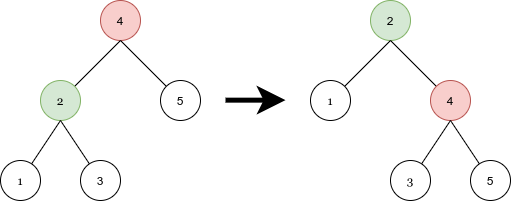
\includegraphics[height=0.3\textwidth]{TreeRotation.png}
\caption{\label{fig2:figs}Visualization of right rotation at node 4. The colored nodes are ones has their \textit{left parent} or \textit{right parent} changed. The \textit{right parent} of node 2, the left child of 4, changed to the \textit{right parent} of 4, and \textit{left parent} of node 4 changed to 2. Left rotation is identical.}

\  
\hrule
\end{figure}

Going to the real life implementation, those changes are only a couple
of lines for each rotation type. The implementations of left and right
rotation are given below.

\begin{lstlisting}
template<class T>
void Treap<T>::leftRotate(Node<T>* &node) {
  Node<T> *parent = node->parent;
  Node<T> *r = node->right;
  node->parent = r;
  node->rightParent = r; // set right parent of the given node
  r->leftParent = node->leftParent; // set left parent of right child 
  if (r->left)
    r->left->parent = node;
  node->right = r->left;
  r->left = node;
  r->parent = parent;
  if (parent) {
    if (parent->left == node) {
      parent->left = r;
    } else {
      parent->right = r;
    }
  }
  node = r;
}
template<class T>
void Treap<T>::rightRotate(Node<T>* &node) {
  Node<T> *parent = node->parent;
  Node<T> *l = node->left;
  node->parent = l;
  node->leftParent = l; // set left parent of the given node
  l->rightParent = node->rightParent; // set right parent of left child 
  if (l->right)
    l->right->parent = node;
  node->left = l->right;
  l->right = node;
  l->parent = parent;
  if (parent) {
    if (parent->left == node) {
      parent->left = l;
    } else {
      parent->right = l;
    }
  }
  node = l;
}
\end{lstlisting}
\vspace{-8mm}

\hypertarget{section2.3}{%
\subsection{2.3. Running time}\label{section2.3}}

Let \(d\) be a difference between \emph{ranks}\footnote{position of the
  value in the sorted array of all values on the tree} of any two node
values on a Treap. Due to Seidel and Aragon \cite{1}, the expected
running time of Finger Search on Treap theoretically is \(O(\log d)\).
Therefore, the closer to the \(finger\) the target value is, the faster
the expected running time will be. Thus, to test and prove if the
running time of Finger Search in practice is identical to the theory,
the search value would be chosen based on a given \(d\).

At first, the Treap is initialized with \(5\,000\,000\) nodes that
contain all values from 1 to \(5\,000\,000\), so it is easy to see that
the difference between \(ranks\) of two nodes are exactly the difference
between their values. The chosen values of \(d\) for testing starts from
a small value (20) and is doubled when \(d\) increases, specifically let
\(D = [20, 20\cdot2^1, 20\cdot2^2, \ldots, 20\cdot2^{15}]\). The testing
program will do the following procedure: \vspace{-4mm}

\begin{enumerate}
\def\labelenumi{\arabic{enumi}.}
\tightlist
\item
  Picks a random node in the Treap and set it to be the \(finger\).
\item
  For each \(d\) in \(D\): \vspace{-4mm}
\end{enumerate}

\begin{quote}
\begin{itemize}
\tightlist
\item
  Repeat \(5\,000\,000\) times: search for a value \(finger + d\) or
  \(finger - d\) which is chosen randomly in the two. Each time a node
  is found, the \(finger\) is set to that node.
\item
  Calculate the average running time of the trials. \vspace{-3mm}
\end{itemize}
\end{quote}

See figure \ref{fig:TreapResult} below for the result data.

\begin{figure}
\centering
\begin{minipage}{1\textwidth}
  \centering
    \begin{tabularx}{0.8\textwidth}{|>{\centering\arraybackslash}X|>{\centering\arraybackslash}X|>{\centering\arraybackslash}X|}
  \hline
      $d$  & Finger Search time  & Binary Search form root time \\ \hline
     20  & 7.89250  & 27.2041 \\ \hline
     40  & 9.95326  & 28.0649 \\ \hline
     80  & 11.9180  & 28.8736 \\ \hline
    160  & 13.9715  & 27.4262 \\ \hline
    320  & 15.8764  & 28.0812 \\ \hline
    640  & 18.3024  & 29.7978 \\ \hline
   1280  & 20.2644  & 29.4003 \\ \hline
   2560  & 22.3453  & 28.0397 \\ \hline
   5120  & 24.6583  & 28.8494 \\ \hline
  10240  & 26.4185  & 28.1270 \\ \hline
  20480  & 28.3653  & 28.4053 \\ \hline
  40960  & 30.1493  & 28.3681 \\ \hline
  81920  & 32.8924  & 28.7313 \\ \hline
 163840  & 33.6583  & 27.9549 \\ \hline
 327680  & 35.6414  & 27.9997 \\ \hline
 655360  & 40.2822  & 27.4228 \\ \hline
  \end{tabularx}
\end{minipage}
\caption[Caption]{Average running time of Finger Search and Binary Search from root on Treap with $d$ in $[20, 20\cdot2^1, 20\cdot2^2, \ldots, 20\cdot2^{15}]$. The total number of search times for each $d$ is $5\,000\,000$. The running times are in \textit{number of nodes visited} at the end of the search function.}
\label{fig:TreapResult}
\end{figure}

\newpage

As you can see, while the running time of Finger Search increases when
\(d\) increases, the usual Binary Search from root remains about the
same for all \(d\), so we can say that Finger Search depends on \(d\).
Obviously, since the time increases about 2 when \(d\) is doubled, see
figure \ref{fig:TreapResult}, the running time of Finger Search is
approximately \(2\log d = O(\log d)\). From that, in the below graph,
the running time for each \(d\) in the graph is divided by \(2\log d\),
denoted \(r_d\) ratio. To see how the running time of Finger Search
related to \(O(\log d)\) in practice, figure \ref{fig:TreapGraph} is
provided below. It is clear that the ratios calculated are almost the
same for all \(d\). This reflects that the running time of Finger Search
is \(O(\log d)\) in practice.

\begin{figure}
\begin{minipage}{0.95\textwidth}
\begin{center}
\begin{tikzpicture}
  \begin{axis}[ 
    symbolic x coords={0, 20, 40, 80, 160, 320, 640, 1280, 2560, 5120, 10240, 20480, 40960, 81920, 163840, 327680, 655360, 1310720},
    xtick={0, 20, 40, 80, 160, 320, 640, 1280, 2560, 5120, 10240, 20480, 40960, 81920, 163840, 327680, 655360, 1310720},
    xticklabels={0,$2^0$,$2^1$, $2^2$,$2^3$,$2^4$,$2^5$,$2^6$,$2^7$,$2^8$,$2^9$,$2^{10}$,$2^{11}$,$2^{12}$,$2^{13}$,$2^{14}$,$2^{15}$,$2^{16}$},
    scaled x ticks={real:20},
    height=5cm,
        width=14cm,
    minor tick num=5,
    grid=both,
    grid style={line width=.1pt, draw=gray!20},
    major grid style={line width=.2pt,draw=gray!40},
    ymin=0,
        ymax=2,
    xmin=0,
        xmax=1310720,
    xlabel=$d$,
    ylabel={$r_d$},
        ylabel style={rotate=-90}
  ] 
        \addplot file[skip first] {TreapGraph.txt};
  \end{axis}
\end{tikzpicture}
\end{center}
\end{minipage}
\caption[Caption]{The graph of ratios $r_d$ versus different values of $d$ given in figure \ref{fig:TreapResult}.}
\label{fig:TreapGraph}
\end{figure}
\hrule

\hypertarget{section3}{%
\section{\texorpdfstring{3. \enspace Finger Search on
Skiplists}{3. Finger Search on Skiplists}}\label{section3}}

\hypertarget{overview-1}{%
\subsection{3.1 Overview}\label{overview-1}}

In this section, we go over the structure of Skiplist and how Finger
Search is performed on it. Skiplist is an interesting and beautiful
structure which uses randomization to optimize the times to search for
an element and some other related operations to \(O(\log n)\). It has a
structure of multiple Linked Lists with common nodes (specifically they
are the same pointers). On each level, each node is randomly determined
if it exists on the next higher level. With this randomized feature,
Skiplist provides a ``magical'' search path that produces \(O(\log n)\)
running time.

With the randomized property, Skiplist supports Finger Seach in
\(O(\log d)\) time. Due to W. Pugh (see \cite{2}), we store the
\(finger\) differently. Other than just one node at a place, we store
the whole ``cover'' from the lowest node to the highest node of the list
that are equal or less than the node at level 1 of the finger. In other
words, the finger is an array of nodes that ``cover'' the bottom-left
corner of the Skiplist from the chosen node. See figure \ref{fig3:figs}
for example.

With this \emph{finger} array, the main idea if Finger Search on
Skiplist due to W. Pugh is: \vspace{-2.5mm}

\begin{itemize}
\tightlist
\item
  If value of the node at the lowest level of the \emph{finger} is less
  than the search value, find the highest level whose node of the
  \emph{finger} has \emph{next} pointer less than the search value.
\item
  If value of the node at the lowest level of the \emph{finger} is
  larger than the search value, find the lowest level whose node of the
  \emph{finger} has \emph{next} pointer less than the search value.
\end{itemize}

From the found level, we start searching normally (on the normal
Skiplist search path) from the \emph{next} node of the \emph{finger}
pointer at that level.

\begin{figure}
\centering
\vspace{1mm}
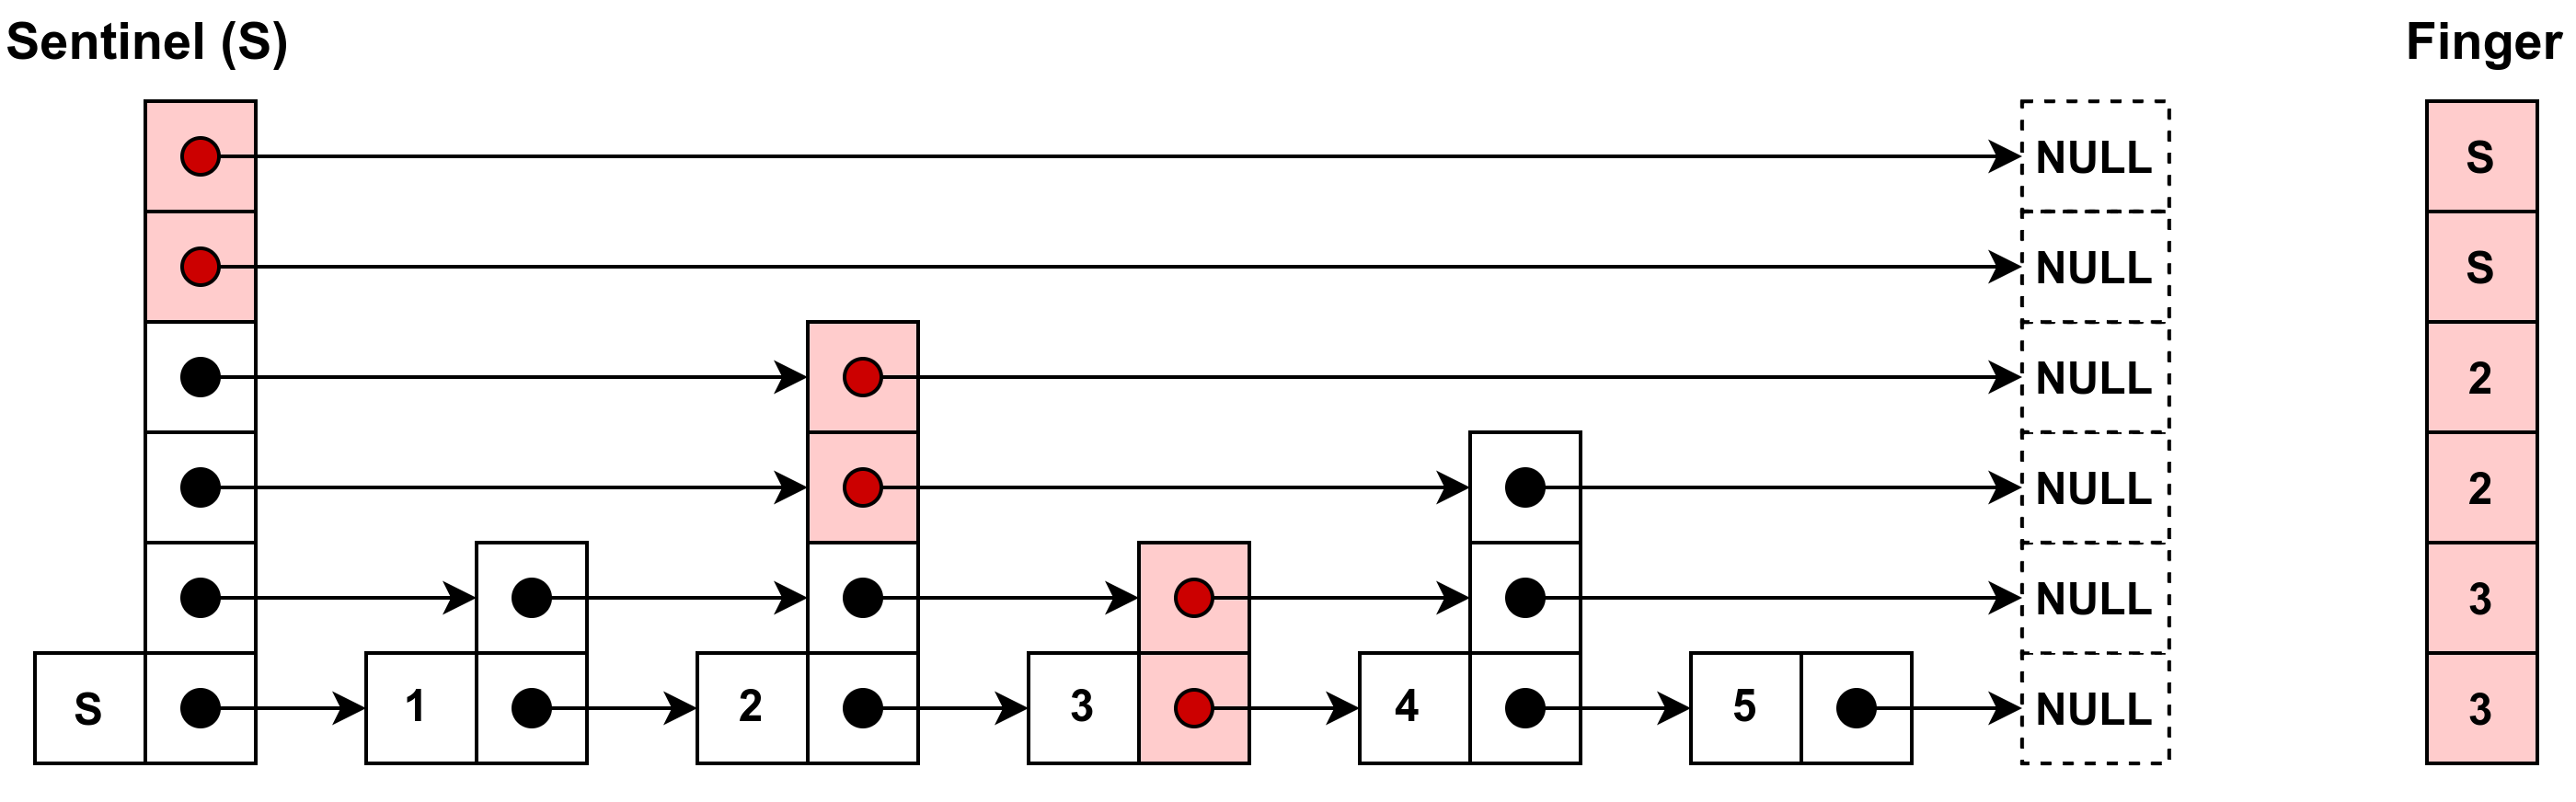
\includegraphics[height=0.3\textwidth]{Skiplist.png}
\caption{\label{fig3:figs}Visualization of a \emph{finger} on a Skiplist. In this example, finger is an array of all nodes cover the bottom-left corner of the Skiplist from node 3.}

\  
\hrule
\end{figure}

\hypertarget{implementation-1}{%
\subsection{3.2. Implementation}\label{implementation-1}}

Due to W. Pugh (see \cite{2}), Finger Search on Skiplist does not
require any additional properties of any other functions or the node
class to perform searching in \(O(\log d)\). Thus, Finger Search is
implemented in its own function without any outside requirements. Let
\(x\) be the search value and assume indices of arrays starts at 1. The
steps of Finger Search on Skiplist is described below:

\begin{enumerate}
\def\labelenumi{\arabic{enumi}.}
\item
  If \(finger[1] < x\), then start from level 2, move upwards until the
  next pointer of current node points to a node larger than \(x\), null
  or the current \(level\) out of bound. At that time, \(level -1\) is
  the level we start searching normally.

  Otherwise, starting from level 2, we also search upwards but until we
  see the first level such that the next node of the \(finger\) at that
  level is less than the search node.
\item
  From the next node of the \(finger\) pointer at the \(level\) found at
  the previous step, perform search as usual (if next node \(< x\), move
  to the \(next\) pointer, otherwise, move down one level until reaching
  the lowest).

  Each time it searches \textbf{down}, set the finger at the current
  \(level\) to the current node to update the \(finger\).
\end{enumerate}

Implementation of Skiplist in this project is provided by Pat Morin, see
\cite{2}. The C++ code is provided below. More error checking is
provided while searching upwards.

\begin{lstlisting}
template<class T>
T Skiplist<T>::fingerSearch(T x) {
  int level = 1;
  Node* start;
  if (compare(finger[0]->x, x) == -1) {
    while (level <= h &&
            (compare(finger[level]->x, x) >= 0
              || (finger[level]->next[level] != nullptr
                  && compare(finger[level]->next[level]->x, x) == -1))) {
      if (compare(finger[level]->x, x) == 0) {
        return x;
      }
      level++;
    }
    start = finger[level]->next[level];
  } else {
    while (level <= h &&
            (compare(finger[level]->x, x) >= 0
              || (finger[level]->next[level] != nullptr
                   && compare(finger[level]->next[level]->x, x) >= 0))) {
      if (compare(finger[level]->x, x) == 0) return x;
      level++;
    }
    if (level > h) {
      level = h;
      start = sentinel;
    } else {
      start = finger[level]->next[level];
    }
  }
  for (int i = level; i >= 0; i--) {
    while (start->next[i] != nullptr && compare(start->next[i]->x, x) < 0) {
      start = start->next[i];
    }
    finger[i] = start;
  }
  return start->next[0] == nullptr ? null : start->next[0]->x;
}
\end{lstlisting}

\hypertarget{running-time}{%
\subsection{3.3. Running time}\label{running-time}}

The running time of Finger Search on Skiplist is identical to Treap. The
concept of distance between \(ranks\) of the lowest node of the
\(finger\) and the search value is applied the same as Treap.
Theoretically, the running time of Finger Search on Skiplist is
\(O(\log d)\), so if the search value \(x\) is closer to the lowest node
of \(finger\), search time would be faster.

The same testing method is used as on Treap: initialize the Skiplist
with \(5\,000\,000\) integers from 1 to \(5\,000\,000\), so the
difference between \(ranks\) of values is the same as the difference
between those values. The testing \(d\) is also
\(\in \{20, 20\cdot 2^1, 20\cdot 2^2, \ldots, 20\cdot 2^{15}\}\), and
using the procedure the same on Treap (see
\protect\hyperlink{section2.3}{Section 2.3} for more details).

\hypertarget{section3.3.1}{%
\subsubsection{3.3.1. Normal running time due to W. Pugh's
approach}\label{section3.3.1}}

The result data with W. Pugh's approach is provided below.

\begin{figure}
\centering
\begin{minipage}{1\textwidth}
  \centering
    \begin{tabularx}{0.8\textwidth}{|>{\centering\arraybackslash}X|>{\centering\arraybackslash}X|>{\centering\arraybackslash}X|}
  \hline
      $d$  & Finger Search time  & Usual search path from Sentinel \\ \hline
     20  & 39.8817  & 44.7127 \\ \hline
     40  & 40.3754  & 41.5027 \\ \hline
     80  & 41.9393  & 41.3186 \\ \hline
    160  & 43.7000  & 41.5630 \\ \hline
    320  & 46.2551  & 43.6607 \\ \hline
    640  & 48.3684  & 44.7823 \\ \hline
   1280  & 48.1796  & 44.3474 \\ \hline
   2560  & 50.3686  & 44.5856 \\ \hline
   5120  & 51.7555  & 43.8798 \\ \hline
  10240  & 53.2053  & 43.3164 \\ \hline
  20480  & 54.6277  & 43.2839 \\ \hline
  40960  & 56.1563  & 43.2849 \\ \hline
  81920  & 57.9879  & 43.4521 \\ \hline
 163840  & 58.7704  & 42.8980 \\ \hline
 327680  & 60.6042  & 43.0317 \\ \hline
 655360  & 63.1080  & 42.6243 \\ \hline
  \end{tabularx}
\end{minipage}
\caption[Caption]{Average running time of Finger Search and Usual search from sentinel on Skiplist with $d$ in $[20, 20\cdot2^1, 20\cdot2^2, \ldots, 20\cdot2^{15}]$. The total number of search times for each $d$ is $5\,000\,000$. The running times are in \textit{number of nodes visited} at the end of the search function.}
\label{fig:SkiplistResult}
\end{figure}
\hrule

~ ~ ~

\vspace{3mm}

As you can see, the running time behaviour of Finger Search on Skiplist
is identical to Treap. It is increasing by about 2 nodes visited when
\(d\) is doubled, so it leads to the running time
\(2\log d = O(\log d)\). The only difference is the running time of
Finger Search on Skiplist is much slower compared to Treap (it starts
from 40 nodes visited while on Treap, it starts from 8 nodes visited),
see Figure \ref{fig:SkiplistResult} and Figure \ref{fig:TreapResult} for
more details.

\hypertarget{running-time-with-additional-concurrent-linear-search}{%
\subsubsection{3.3.2. Running time with additional concurrent linear
search}\label{running-time-with-additional-concurrent-linear-search}}

Additional to the approach of W. Pugh (see \cite{2}), I introduce a
simple concurrent linear search along with Finger Search when we search
upwards or downwards. For every iteration and with a tracking variable,
we perform a linear search (go to the next node or previous node after
every iteration) from the lowest level of the \(finger\) towards the
search value \(x\). This approach is created in the hope of reduce the
running time of Finger Search if the \(finger\) is close to \(x\).

Running time of Finger Search with linear search is provided below.

\begin{figure}
\centering
\begin{minipage}{1\textwidth}
  \centering
    \begin{tabularx}{0.8\textwidth}{|>{\centering\arraybackslash}X|>{\centering\arraybackslash}X|>{\centering\arraybackslash}X|}
  \hline
      $d$  & Finger Search time with linear search  & Usual search path from Sentinel \\ \hline
     20  & 20      & 43.5811 \\ \hline
     40  & 40      & 41.5027 \\ \hline
     80  & 40.8913 & 40.0918 \\ \hline
    160  & 43.3681 & 41.7235 \\ \hline
    320  & 45.2700 & 42.1257 \\ \hline
    640  & 47.6589 & 43.9823 \\ \hline
   1280  & 48.7145 & 44.4602 \\ \hline
   2560  & 49.1672 & 43.8023 \\ \hline
   5120  & 51.0105 & 43.5328 \\ \hline
  10240  & 53.1527 & 44.0019 \\ \hline
  20480  & 54.3721 & 43.4647 \\ \hline
  40960  & 55.8258 & 42.5021 \\ \hline
  81920  & 57.0091 & 44.1179 \\ \hline
 163840  & 60.1422 & 43.0084 \\ \hline
 327680  & 61.7512 & 44.1739 \\ \hline
 655360  & 63.5892 & 44.8285 \\ \hline
  \end{tabularx}
\end{minipage}
\caption[Caption]{Average running time of Finger Search with linear search and Usual search from sentinel on Skiplist with $d$ in $[20, 20\cdot2^1, 20\cdot2^2, \ldots, 20\cdot2^{15}]$. The total number of search times for each $d$ is $5\,000\,000$. The running times are in \textit{number of nodes visited} at the end of the search function.}
\label{fig:SkiplistLinearSearchResult}
\end{figure}
\hrule

~ ~ ~

\vspace{3mm}

It is obvious that the linear search helps improve running time
searching for a value very close to the \(finger\). As long as the
Finger Search path to the value is longer than the \(ranks\) between
them, the linear search reduce the search time equals to the difference
in \(ranks\). However, when \(d\) gets larger, Finger Search remains
search time \(O(\log d)\) while the linear search is \(O(d)\), so the
larger \(d\) gets, the faster Finger Search is compared to linear
search. As you can see in Figure \ref{fig:SkiplistLinearSearchResult},
with \(d \in \{20, 40\}\), Finger Search time is equal to \(d\) (which
is the linear search time) while if \(d\in\{80, 160,\ldots, 655360\}\),
running time of Finger Search is less than \(d\) (which is the normal
Finger Search time). Since there is only a small portion of \(d\) in
which linear search is faster, we can conclude that the addition of it
in Finger Search is not useful, and it does not reflect and have any
contribute to the consistent \(O(\log d)\) running time of Finger
Search.

\hypertarget{finger-search-on-treaps-and-skiplists-comparison}{%
\section{4. Finger Search on Treaps and Skiplists
comparison}\label{finger-search-on-treaps-and-skiplists-comparison}}

\hypertarget{running-time-1}{%
\subsection{4.1. Running time}\label{running-time-1}}

In theory, since both Treap and Skiplist are randomized data structures,
they are very suitable for Finger Search. With that property, they
produce search time \(O(\log d)\) with \(d\) is the difference between
\(ranks\) of the \(finger\)'s value and the search value. In practice,
the running time of both reflect the \(O(\log d)\) time. Specifically,
times search on both structures increase by about 2 in average when
\(d\) is doubled. This is consistent for both randomized data structure.
However, when we compare them, the time of Finger Search on Treap is
much faster, see \protect\hyperlink{section3.3.1}{Section 3.3.1} and
\protect\hyperlink{section2.3}{Section 2.3} for detailed data.

\hypertarget{implementation-difficulties}{%
\subsection{4.2. Implementation
difficulties}\label{implementation-difficulties}}

Although all data structures have the same idea about Finger Search,
implementation of each data structure is very different from the others.
Through implementations of Finger Search of Treap and Skiplist, to me,
the easier one is Treap. Even I needed to change some functions other
than the new Finger Search function, while the only change in Skiplist
is the new search function, the implementation of Finger Search on Treap
is very simple compared to Skiplist.

On Treap, changing the rotation functions takes only two lines and easy
to keep track. For the Finger Search function, I did not need
complicated error checking for special cases since they are
automatically excluded in Finger Search. Therefore, the implementation
is straightforward and even shorter.

On Skiplist, there are cases that the \(next\) pointer is \(null\) or
the pointer is going out of the list. To handle these cases, error
checking is needed in the function. In addition, since the \(finger\) is
not just a pointer while it is an array in Skiplist, changing between
different level is needed and and it is more complicated compare to
Treap while it just compares the value of the pointer with current
node's value.

\hypertarget{concluding-remarks}{%
\section{5. Concluding remarks}\label{concluding-remarks}}

Finger Search and its implementations has been described detailedly in
the report. Its performance is exactly as theory as producing running
time \(O(\log d)\). There are several conclusions regarding to Finger
Search in the real life:

\begin{enumerate}
\def\labelenumi{\arabic{enumi}.}
\tightlist
\item
  The algorithm's searching approach is not the same for every data
  structure. Each of them has its own implementation and running time.
\item
  For both Treap and Skiplist, Finger Search runs in \(O(\log d)\).
  Specifically, it is \(\approx 2\log d\) while the running time
  increases by 2 if \(d\) is doubled.
\item
  Finger Search on Treap is much faster than on Skiplist.
\end{enumerate}

\newpage
\begin{thebibliography}{9}
\bibitem{1}
Seidel, R., Aragon, C.R. Randomized search trees. \emph{Algorithmica} 16, 464–497 (1996). \url{https://doi.org/10.1007/BF01940876}
\bibitem{2}
W. Pugh. \emph{A skip list cookbook}. Technical Report CS-TR-2286.1, Dept. of Computer
Science, University of Maryland, College Park, 1989.
\bibitem{3}
Morin, P. (2014). \emph{Open Data Structures}. Edmonton: Athabasca University Press.
\vspace{-1.5mm}

\url{https://opendatastructures.org/}

\end{thebibliography}

\end{document}
